\chapter{A térkép}
A pálya aktuális térképe a \ref{fig:stalingrad}. ábrán látható.

\begin{figure}
    \centering
    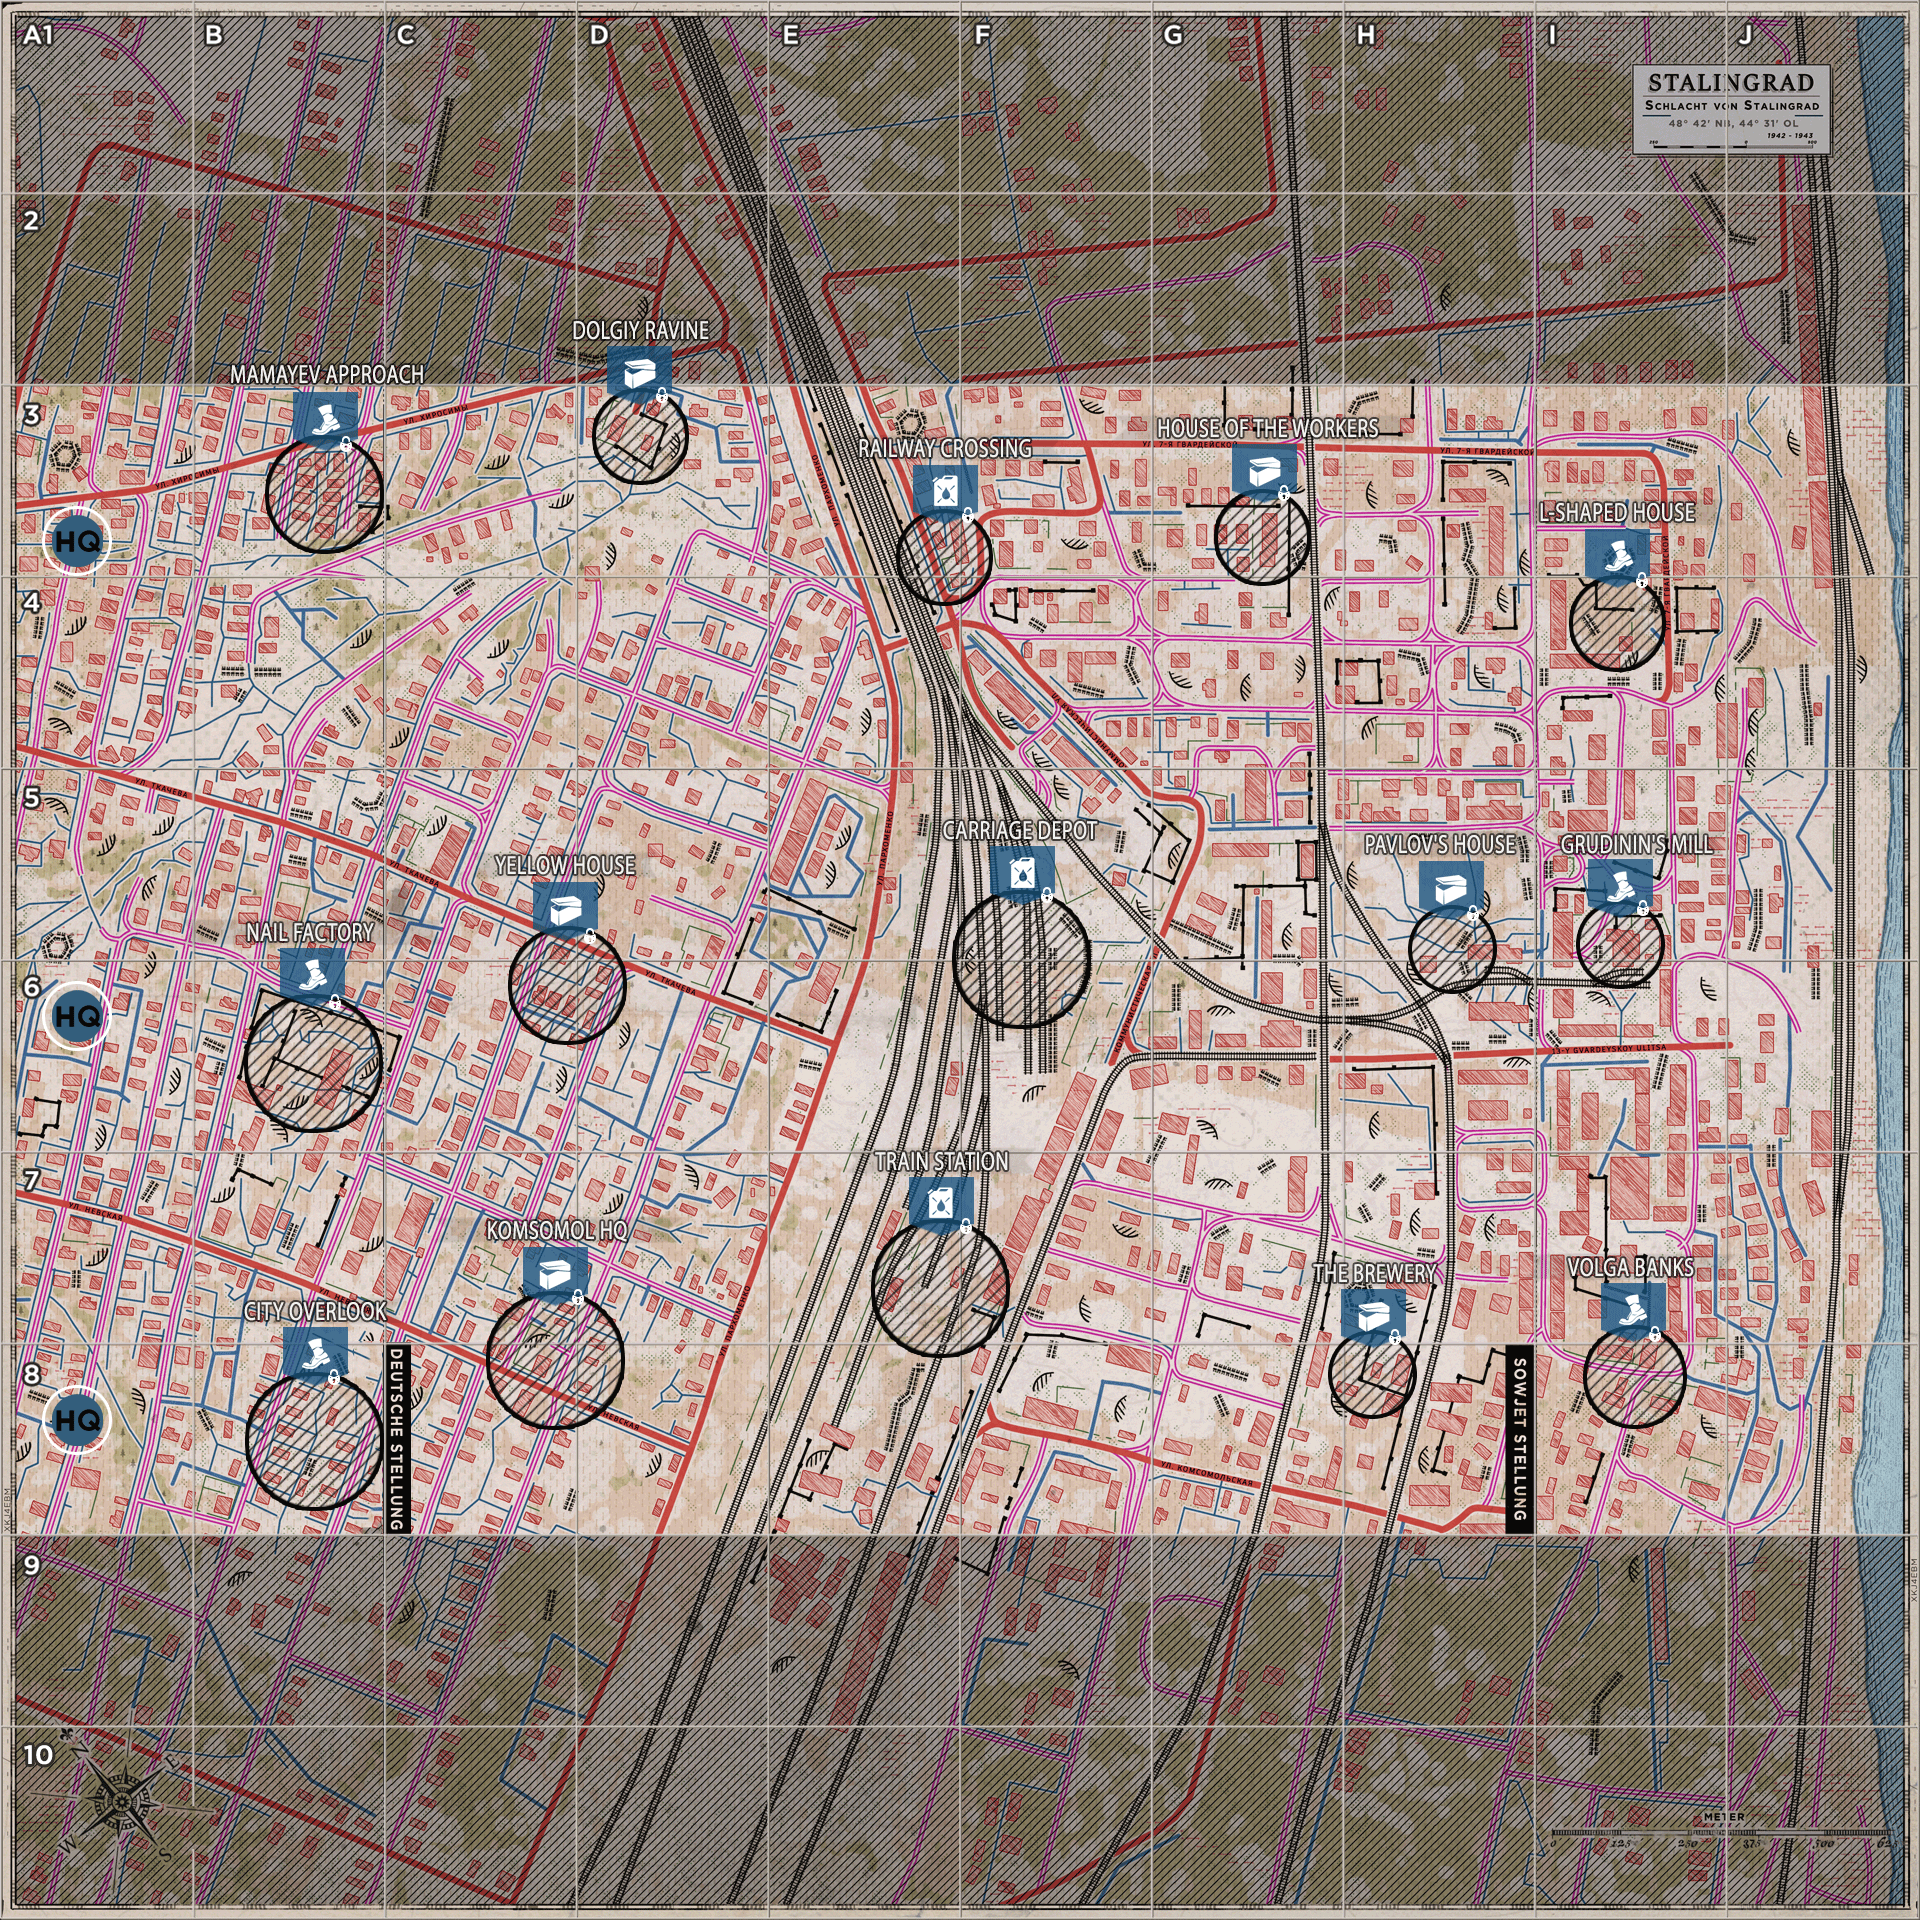
\includegraphics[width=150mm, keepaspectratio]{figures/StalingradMap.png}
    \caption{Sztálingrád térképe}
    \label{fig:stalingrad}
\end{figure}

%-------------------------------------
\section{Német bázis sáv}
%-------------------------------------
\subsection{Mamayev Approach}

\subsection{Nail Factory}
A terület 2-3 gyárépülettel tagolt, de az is pár faltól eltekintve a földdel egyenlő. Nagyon könnyen védhető minden irányból.

\subsection{City Overlook}

%-------------------------------------
\section{Német védekező sáv}
%-------------------------------------
\subsection{Dolgiy Ravine}

\subsection{Yellow house}
Néhány ház található itt, magas kerítésekkel. Nehezen védhető pont.

\subsection{Komsomol HQ}

%-------------------------------------
\section{Semleges sáv}
%-------------------------------------
\subsection{Railway Crossing}

\subsection{Carriage Depot}
A vasútállomás. Az egyik legnyíltabb terepnek mondható. Kevés fedezék található a területen, szinte csak a vagonok nyújtanak menedéket, de azokból van sok. 

Német oldalon a pont mögötti magaslat miatt tankkal jól belátható.

\subsection{Train Station}

%-------------------------------------
\section{Orosz védekező sáv}
%-------------------------------------
\subsection{House of the Workers}

\subsection{Pavlov's House}

\subsection{The Brewery}
Sok romház található a környéken. Egyészen jól védhető. Ha a védő csapat jól be tudja ásni magát vagy jó pozíciókat tud felvenni, akkor sokáig visszaverhető a támadás.

%-------------------------------------
\section{Orosz bázis sáv}
%-------------------------------------
\subsection{L-Shaped House}

\subsection{Grudinin's Mill}
Rengeteg romos épület. A szovjetek könnyen meg tudják rohamozni és befoglalni a játék elején.

\subsection{Volga Banks}